\documentclass[12pt]{article}


\usepackage{amsmath}	% The ''amsmath'' package will allow you to use useful 
					% commands contained within the AMS-LaTeX package.
					% (AMS is the American Mathematical Society.)
					
\usepackage{amssymb}		% The ''amssymb'' package will allow you to use 
						% additional mathematical symbols.
						
\usepackage{amsthm}		% The ''amsthm'' package contains commands
						% for formatting mathematical theorems and 
						% statements.
						

\usepackage{graphicx}
\usepackage{url}
\usepackage{setspace}
                                        
\usepackage{enumitem}                                                                          
       
                  
                                                                            
\usepackage{graphicx}
\graphicspath{ {images/} }
                                        
\usepackage[top=.5in,bottom=1in,left=1in,right=1in]{geometry}	
          





% Now we begin the BODY OF YOUR DOCUMENT:

\begin{document}	% All LaTeX files contain the command ''\begin{document}''. 
				% There is a corresponding ''\end{document}'' command
				% at the end.

% Next we'll give basic titling information to LaTeX:


% use to insert a blank page: \clearpage\thispagestyle{empty}\null\clearpage


% \title{Junior IS}	% The title of the document.

% \author{Avery Rapson}			% The author

% \date{\today}		% This date-stamps your paper automatically. If you want to 
				% specify a fixed date, you may do so between the braces.
				% If you don't want a date to appear, type ''\date{}''.

% Creating the title section:

% \maketitle		% This command creates the appropriate header. It may alternatively
			% create a title page. This will depend on whether you have selected  
 			% ''report'', ''book", or ''article'' in the ''\documentclass'' command above.
			

\doublespacing		% The ''\doublespacing'' command is available only if
					% ''\usepackage{setspace}'' is in the document. This 
					% causes the document to be double-spaced (surprise!).
					
					
%%%%%%%%%						
%  Start Paper  %
%%%%%%%%%	
				
				
				
%Creating the illusion of virtual reality

%How the senses contribute to that illusion

%How these senses are implemented through enabling hardware. 

% virtual systems that implement human senses into the simulation


\includegraphics[width=\textwidth]{cover}

\pagenumbering{gobble}
\clearpage
\setcounter{page}{1}

\pagenumbering{arabic}

\tableofcontents


\newpage


%%%%%%%%%						
%    Section 1   %
%%%%%%%%%

\section{Introduction}
The largest problem in the virtual reality (VR) industry is achieving successful immersion. To understand and come up with a solution to this problem, it is important to identity the factors that contribute to a successful immersive virtual experience. The next step is evaluating the theory behind successful immersion and speculating how one could transfer that knowledge into making VR applications.  After giving a brief history of VR and its many applications, this paper describes the factors that go into creating successful immersion and speaks on the hardware and software that bring VR to life.
A VR application is then created after learning more about VR and Unity 5. The goal of this project is to put this theory into practice by building and running a mobile VR scene on the Google Cardboard headset. 

\subsection{Defining VR}
VR is a term that is being used more and more in today's society, become the new hot topic. The increasing development of so many different VR systems has caused people to form their own impressions of what VR really is and how it is defined. Therefore, it is important give a formal definition of VR, and describe how it is accomplished. A formal definition of a virtual reality is as follows: 

\begin{quote}
A medium composed of interactive computer simulations that sense the participant's position and actions, providing synthetic feedback to one or more senses, giving the feeling of being 
immersed or being present in the simulation \cite{craig}. 
\end{quote}

In order to create a virtual reality, a virtual world must be presented that appeals to our senses the same way people perceive reality. VR's singular goal is to display an illusion so successful that the user believes they are somewhere else entirely. 



\subsection{History and Origins}


Although VR seems like a fairly new science, the concept stretches all the way back to the 1930's. Alders Huxley and Stanley Weinbaum wrote books imagining movies that extend past just sight and sound to include taste, smell and even touch \cite{mihelj}. These sensory additions work to displace the viewer from their current reality and immerse them in another. 

 
\par The first concepts of VR were brought to life around 20 years later by a man named Morton Heilig. Heilig created a machine called the \textit {Sensorama}, which offered a virtual bicycle riding experience \cite{mihelj}. This machine enabled the user to observe a three-dimensional display while listening to sounds of a city and experiencing the wind, vibrations and even smells that one would experience on a real bike ride.

   \begin{figure}[h]
         \centering
    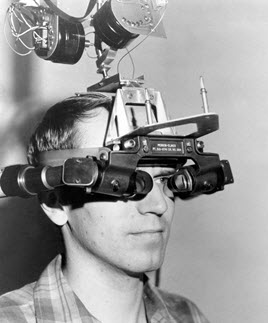
\includegraphics[width=0.4\textwidth]{photo1_sutehrland}
    \caption{Sutherland's Head Mounted Dispay \cite{photo1_sutehrland}}
    \label{fig:sutherland_Display}
 \end{figure} 
 \par In 1976, this innovative technology led Ivan Sutherland to create the first head mounted display that was connected to a virtual environment, seen in figure \ref{fig:sutherland_Display}. Similar to modern virtual hardware, Sutherland's display consisted of glasses with two small screens that created the illusion of three-dimensional vision. The display allows the user to change what they observed by moving their head. This technology required a complex motion tracking system attached to the ceiling. Although groundbreaking, Sutherland's device did not let the user to interact on any level with the virtual environment.

  \par Even though the technology did not exist, Sutherland had a vision of an ultimate stage of VR development, and how it could be achieved. A challenge was set that has motivated the progress of VR ever since: 
  
 \begin{quote}
The screen is a window through which ones sees a virtual world. The challenge is to make that world look real, act real, sound real, and feel real  \cite{gobbetti}. 
\end{quote}

The challenge was accepted by a man named Myron Kreuger, who coined the term artificial reality around 1970. Krueger created the first virtual system that allowed a user to interact with objects in a virtual environment. Through various sensors, the user's activities were monitored, allowing feedback within the program. Virtual object interaction was a huge advancement towards completing Sutherland's challenge and inspired many new technologies to follow suit.  

Since Kreuger, VR development has continued to grow and become more popular, seeing many new innovations. VR in the media played a huge part in the popularization of the term. Movies like Tron and the Matrix imagined virtual worlds so advanced that distinguishing them from reality became nearly impossible. Though VR technology progress  continued through the 70's and 80's, Sutherland's challenge had only been achieved through film and imagination. 
In the 1990's, the Cave Automatic Virtual Environment, or CAVE was created. 
 \begin{figure}[h]
    \centering
 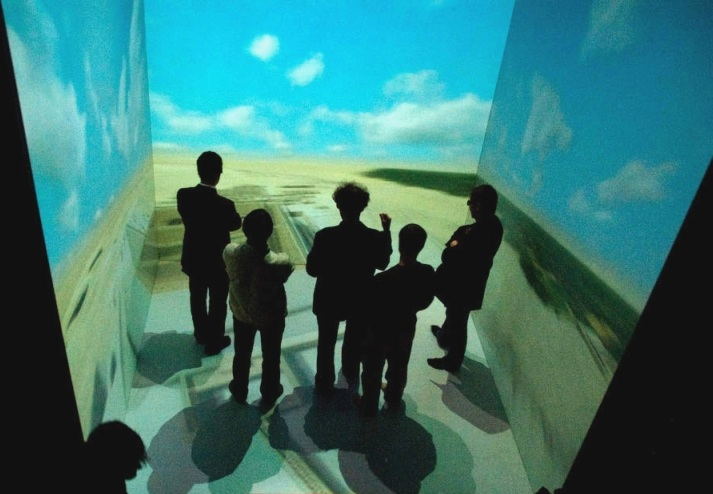
\includegraphics[width=.55\textwidth]{photo16_cave}
  \caption{CAVE: 4 Screens With 4 Stereoscopic Projectors \cite{CAVE}}
  \label{fig:cave}
 \end{figure}
CAVE was a large room full of screens that displayed a virtual environment, taking a different approach to VR hardware \cite{mihelj}.One could also wear special glasses that made objects seem more three-dimensional in the eyes of the user. Special sensors and surround sound were also built to promote immersion and multiple users could fit in a Cave, enabling collaboration. In just 60 years, the concept of VR was born and turned into a reality. Today, perfectly immersive virtual worlds have yet to be achieved, but the advancements and uses of VR have reached heights previously thought impossible. 


  
\subsection{Current Applications and Emerging Markets}
VR enables people's imaginations to run wild. Although the age of consumer VR is just starting to blossom, the range of applications is tremendous. One of the most commercially popular areas of VR is within the gaming industry. VR has the potential to change gaming as we know it. The potential for deep immersion, virtual presence and the production value that VR has to offer is driving developers and manufacturers to take part in the emerging field \cite{parisi}.   


\par However, VR is no longer just for entertainment, having many practical applications as well. Different types of simulators have become the best-known practical application for VR. For example, VR has the potential to become very influential for simulations involving military training, medical training, design and engineering. 

 \begin{figure}[h]
    \centering
 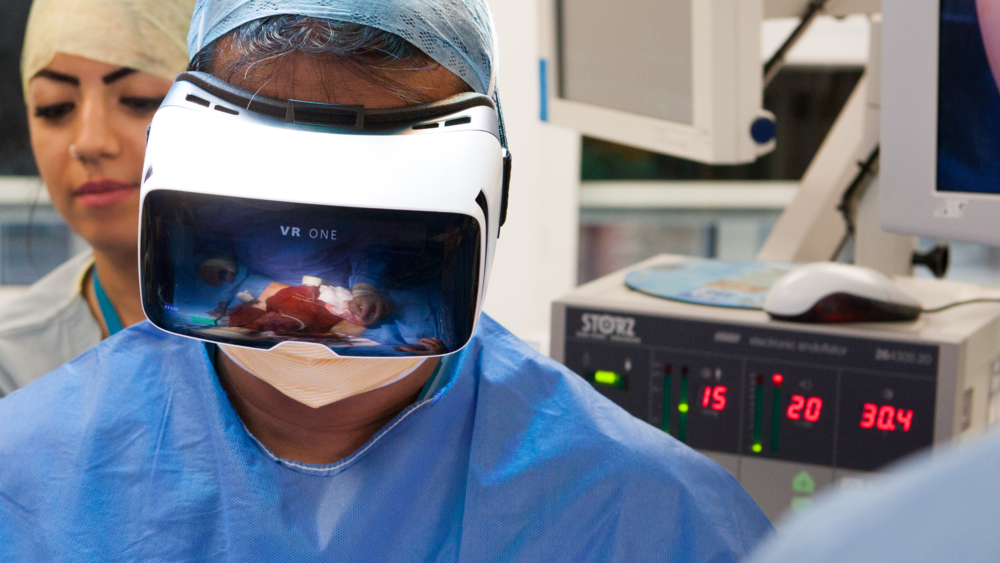
\includegraphics[width=.6\textwidth]{photo2_health}
  \caption{VR Medical Applications \cite{applications}}
  \label{fig:applications}
 \end{figure}
 
These examples are just the beginning. The potential for VR in modern society is endless,  ranging from interactive tourism to psychotherapy.
With more and more foreseeable applications in todays society, the demand and technological innovations will just continue to increase, making VR development society's next big emphasis.  \\




%%%%%%%%%						
%    Section 2   %
%%%%%%%%%

\section{Creating the Illusion of VR}

\subsection{Virtual Presence}

VR is a unique form of media quite unlike other medias such as books or movies and should be dealt with as such. To acquire virtual presence while reading a book, a reader must leave his current reality behind to enter the reality they are reading of \cite{mihelj}. VR requires the opposite. With VR, the user is placed into an environment and is meant to perceive and to respond to it as though it were real. Virtual presence is the feeling of actually existing within a a virtual environment. In the words of Albert Einstein, reality is merely an illusion, albeit a very persistent one. Creating a successful virtual environment requires the creation of a successful illusion.  An effective illusion is made possible through a strong virtual presence. Virtual presence is achieved mentally, physically, or a combination of the two. 

\subsubsection{Physical Presence}

%The simulation, or virtual environment is the first step to building a successful virtual reality. 
Physical presence is an essential part of VR and takes place when the user's body physically enters the simulation or environment. It is what truly sets VR apart from other media.  In response to the users actions, select stimuli are presented to the user which affect perception of the environment. Specifically, virtual environments are described through sight, sound and touch. These sensory perceptions define user interaction in a virtual world and are described in greater detail in the following section. 
 
 \par The goal to obtaining optimal virtual presence is reducing as much real world stimuli as possible.
 After being immersed in the environment, virtual stimuli work to replace the user's exposure of real stimuli, decreasing mental and physical presence in the real world. Physical and mental presence go hand in hand. If physical stimuli are tricked to make you think you are present in a different environment, your mental presence in that environment also increases. 
 
 
 \begin{figure}[h]
    \centering
 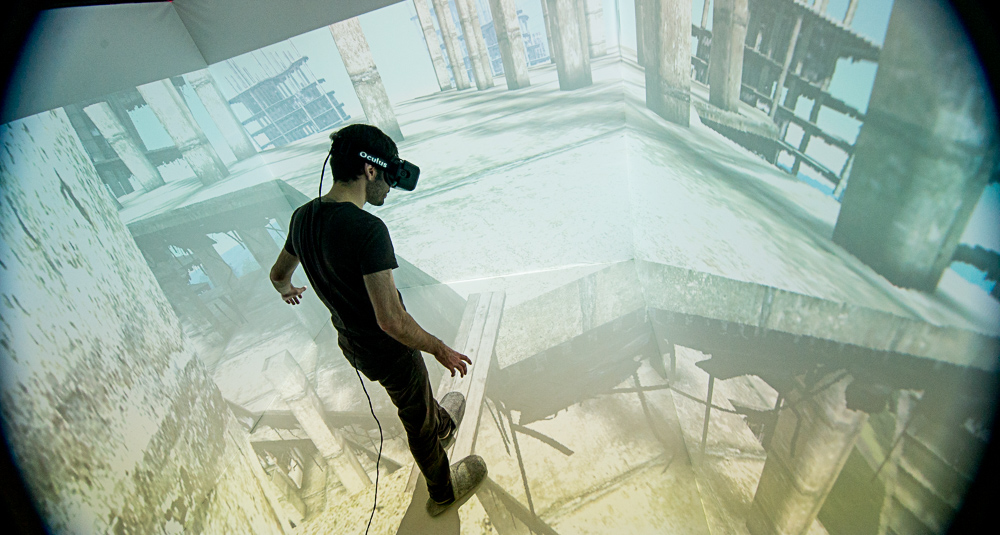
\includegraphics[width=.7\textwidth]{photo15_presence}
  \caption{Virtual Presence: Inducing A Fear of Heights \cite{CAVE}}
  \label{fig:virtualPresence}
 \end{figure}
 
 \subsubsection{Mental Presence}
 
It is possible for a user to be so immersed in a virtual world that it becomes their reality. Mental presence is the non-physical state of engagement felt after entering a virtual world. A realistic display is defined in terms of sight, sound and touch. Achieving and maintaining mental presence is a very delicate and complicated process. There are many factors that affect mental presence. This also means many factors can destroy an immersive process. For example, a sense of virtual realism can be destroyed by small environmental defects because they distract the user from perceiving the scene as legitimate. The level of mental  presence is affected by the virtual scenario, the quality of realism, the number of senses stimulated, and the delay between the users actions and its effect on the virtual world. Mental presence within a virtual reality is difficult to achieve because all of these factors must be taken into account. In order to  successfully obtain virtual presence, a minimum level of physical and mental presence is key.  

\subsection{Human interaction in Virtual Environments}
 VR is created through an exchange of information with the user and the virtual environment. For VR to be realistic, there must be a certain degree of responsiveness to a users actions or inputs. Interaction within a virtual environment can be broken down into three categories: manipulation, navigation and communication. 
Manipulation allows the user to interact and make modifications to the virtual world and the objects it possesses. This interaction increases mental presence within an environment by promoting creativity and expression. Navigation permits the user to maneuver through the world, giving an illusion of depth within an environment. Effective navigation techniques require the user to create a mental picture of the environment, inherently promoting mental presence. Communication enables interaction between users and intermediaries in a virtual environment. Having multiple users in an environment enables an exchange of information and experiences \cite{mihelj}.


%%%%%%%%%						
%    Section 3   %
%%%%%%%%%

\section{Sensory Perception and Enabling Hardware} %maybe sensory inputs and devices/hardware?
In everyday life, we use our senses to pick up stimuli in order to construct a notion of physical reality. To create a successful virtual environment, a similar notion of physical reality must be constructed. In order to forge the existence of a synthetic reality, a virtual system's outputs must correspond to the human senses. The senses most valuable to virtual presence include vision, touch and force perception, hearing, smell and taste \cite{gobbetti}. %page 7
It is therefore crucial to understand sensory stimulation and its significance pertaining to a sense of immersion in a virtual system. The following sections focus on visual, sound and haptic perception.

% for citing, should i say the following research on sensory perception  comes from article X?

\subsection{Visual Perception}

Visual perception is considered to be the most dominant sense. This is demonstrated by the fact that the visual system is given precedence over the other senses when conflicting inputs are present \cite{gobbetti}. Because human behavior is so visually oriented, visual representation is given the highest priority within virtual environments.


\par Depth perception, field-of-view, and critical fusion frequency play important roles within a virtual display. Depth perception is a human's primary tool for observing depth. The complete field of view for human eyes is around 180 degrees horizontally, and over 120 degrees vertically. 
\begin{figure}[h]
    \centering
 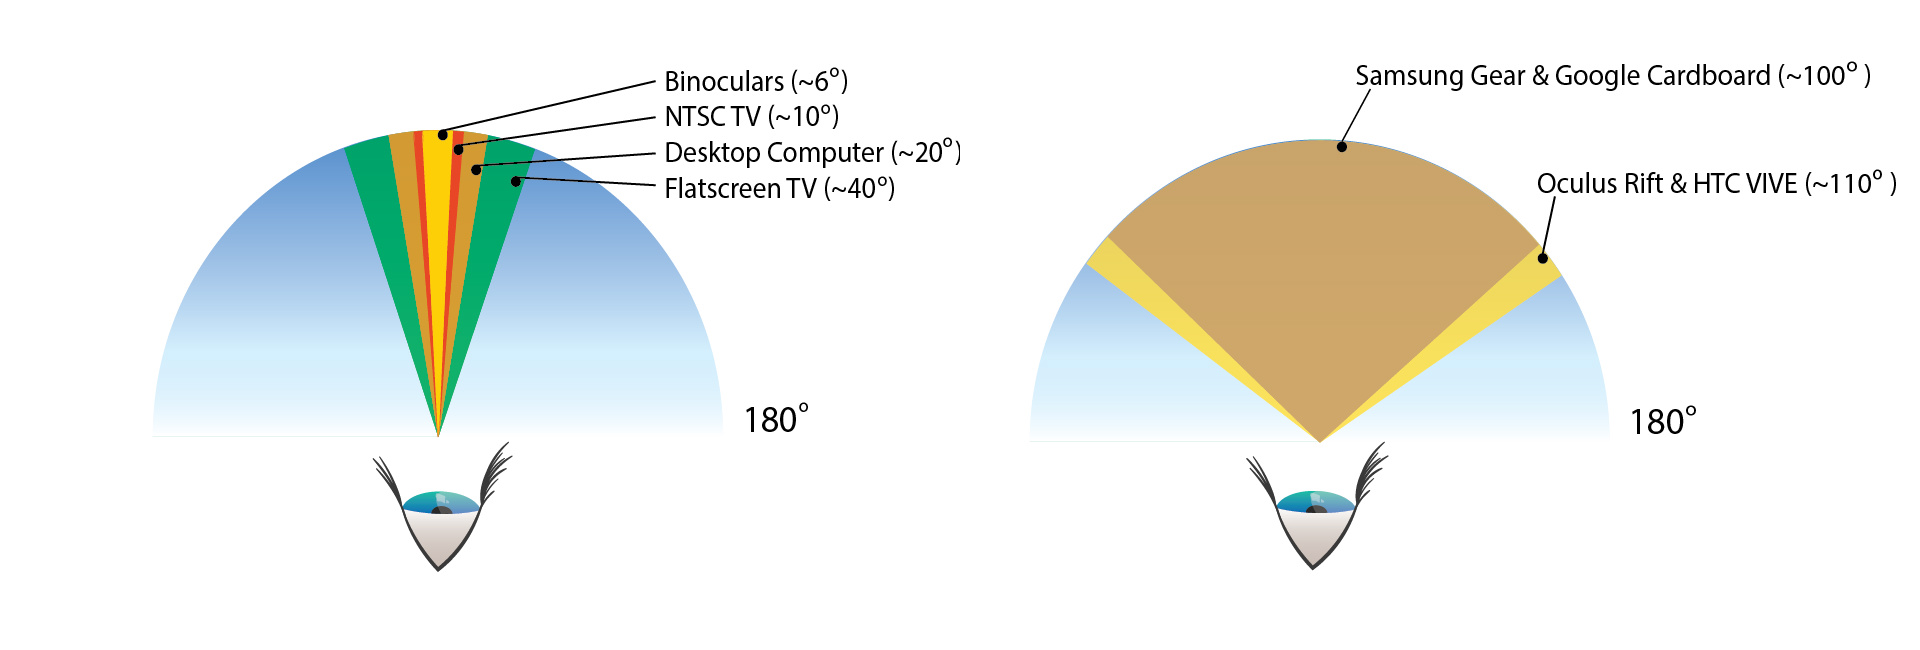
\includegraphics[width=\textwidth]{photo7_fov}
  \caption{Field of View Comparisons \cite{pov}}
  \label{fig:fieldOfView}
 \end{figure}
 
This is important to realize because to accomplish optimal virtual presence, between 90 to 110 degrees are necessary for the horizontal field of vision \cite{gobbetti}. The critical fusion frequency is the rate that humans can distinguish between successive visual stimuli. For example, with a frequency too small, objects will cease to appear as if they are in continual motion, becoming choppy. In computer graphics, a rate below 30-60 Hz results in these effects. Factors such as these result in  distraction and a reminder the user of their presence in a virtual setting. 

\par Given the significance of the visual system, visual displays have become the most important piece of VR hardware. Figure \ref{fig:oculus} displays the oculus rift, an example of commercially popular head tracking hardware. The ability to track head movements and update a visual display accordingly is extremely effective in promoting a virtual presence. Visual displays require stereoscopic vision and must deliver stimuli of acceptable resolution, high-quality motion representations and satisfactory levels of brightness \cite{gobbetti}. 


\begin{figure}[h]
    \centering
 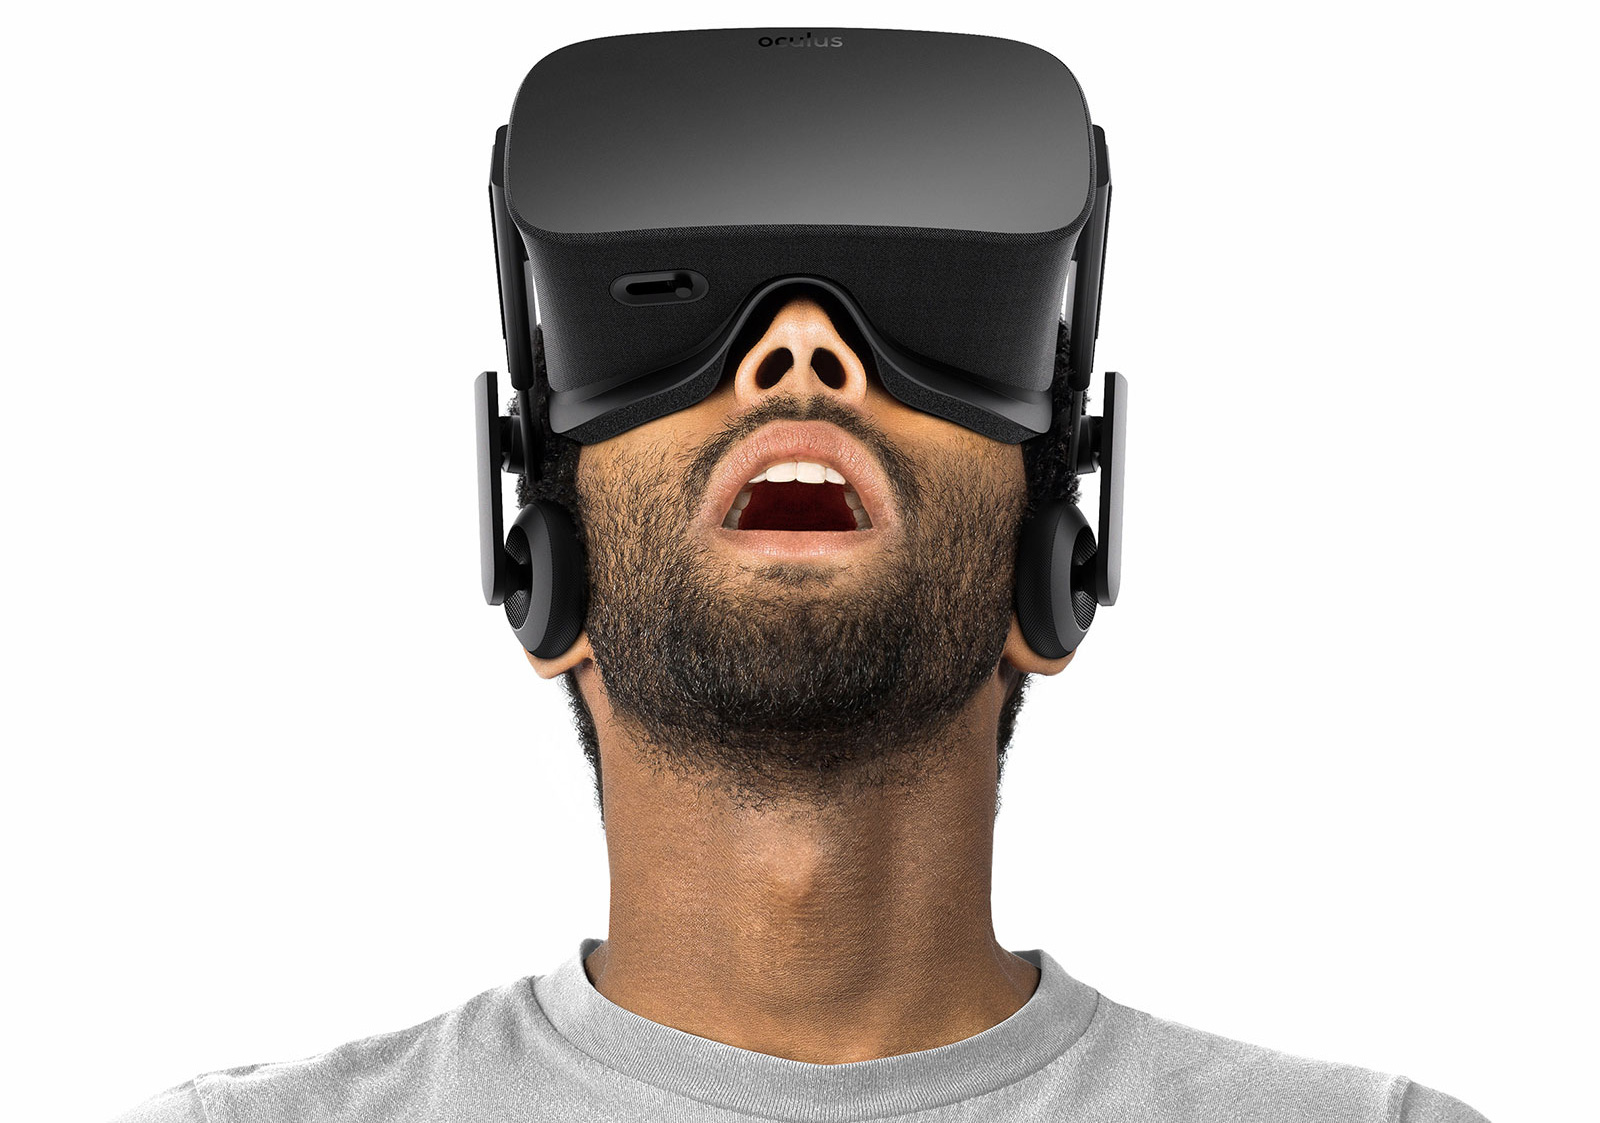
\includegraphics[width=.65\textwidth]{picture11_oculus}
  \caption{Head Mounted Display: The Oculus Rift \cite{oculus}}
  \label{fig:oculus}
 \end{figure}


\subsection{Sound Perception}
While vision is primarily used for virtual perception, the use of sound is invaluable. Hearing and sound perception allow for verbal communication. Verbal communication increases situational awareness, cues visual attention and presents complex information that vision cannot always provide.  Audio perception therefore requires the ability to synthesize sound and to locate and pinpoint auditory stimuli within a 3D space. The most efficient hearing frequency  in humans occurs between 1000 and 4000 Hz \cite{gobbetti}. %[quote page 8]

 
\par Within a virtual environment, auditory stimuli can be generated using location-dependent filters to enhance a users virtual presence. In such environments, stereo, or auditory, clues can be given for users to evaluate. These stereo clues can exist for users to make assumptions on elevational changes or to determine directivity. The challenge for auditory implementation in virtual environments stems from the complexity of auditory perception, illustrated in figure \ref{fig:soundPerception}. Auditory processing is often overlooked in virtual settings due to the complexity of implementation.

\begin{figure}[h]
    \centering
 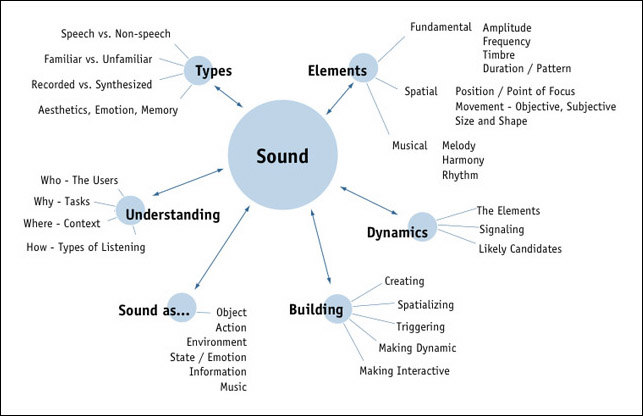
\includegraphics[width=.7\textwidth]{photo8_sound}
  \caption{The Complex Nature of Auditory Processing \cite{sound}}
  \label{fig:soundPerception}
 \end{figure}

\subsection{Haptic Perception}
Haptic perception is unique from vision and sound because it provides the ability to sense and also act upon an environment.
 Through touch, different types of information can be gathered when manipulating different types of objects. The information gathered can be characterized as either tactile or proprioceptive \cite{gobbetti}. Tactile information is gathered from an initial touch of an object. This provides knowledge of the shape and the texture of the object. Applying extended force to an object provides proprioceptive information of the objects weight, forces acting upon the object and surface compliance \cite{gobbetti}. %[quote 9]
Combining tactile and proprioceptive cues allow the user to feel present and engaged within a virtual setting.

\par There are several haptic systems that exist. Gloves are an example of a popular haptic system, shown in figure \ref{fig:hapticPerception}. Other haptic systems that are popular resemble handheld devices similar to a Wii remote. Since haptic perception is so complex, these systems are less common than visual and aural systems. In VR systems, force feedback must measure user movement and sense any exerted forces. They must then calculate the effect of the exerted force upon objects and respond accordingly with resultant forces upon the user's fingers, wrists, or arms \cite{gobbetti}.

\begin{figure}[h]
    \centering
 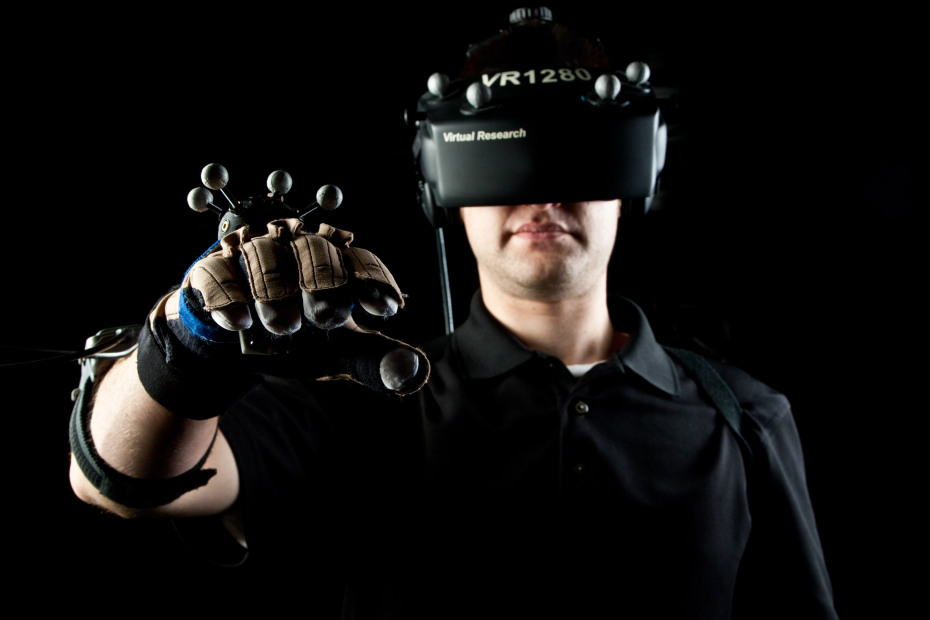
\includegraphics[width=.55\textwidth]{picture12_haptics2}
  \caption{Haptic Gloves \cite{haptics}}
  \label{fig:hapticPerception}
 \end{figure}





%%%%%%%%%						
%    Section 4   %
%%%%%%%%%



\section{Unity}

This project requires a better understanding of Unity. The following sections give a basic overview of Unity, and how VR is created within the game engine. 

\subsection{What Unity has to Offer}

Unity is a professional game engine that is used to create video games and virtual environments for a variety of platforms. Unity has two distinct advantages over other game development environments. The first is Unity's extremely user friendly visual workflow. Other game development tools are often overly complicated and require the user to set up their own integrated development environment, or IDE. Unity's visual editor is both sophisticated and extremely productive, allowing high quality games to be produced with relative ease and efficiency. The second advantage is Unity's wide array of cross-platform support. There are very few game engines that offer as many deployment targets, ranging from the PC, web and mobile to consoles. Unity also makes deploying to these platforms extremely simple. Compared to other game engines such as Unreal, CryEngine, or Game Maker, Unity stands in a fantastic middle ground in terms of the difficulty to learn and desired capabilities in engines. These comparisons and characteristics are brief examples of what makes Unity the engine of choice for many developers.

\subsection{Unity's User Interface}

Unity's user interface is split up into different tabs and sections, shown in figure \ref{fig:UnityUI}. The Project tab is used to view and access all the files in your project and the Console tab is available to view the output from your code. The Scene tab allows you to view the objects placed into the 3D scene and the Game tab lets you view the 3D scene as though the game is being played. The Hierarchy tab shows a list of all the objects in the scene and how they are nested in relation to each other. The Inspector tab displays information about the object selected and lets you change different components. The Toolbar provides scene navigation, including Move, Orbit, and Zoom functions. Unity's interface allows the user to easily create a 3D scene, however scripting is what brings a project to life. 

\begin{figure}[h]
    \centering
 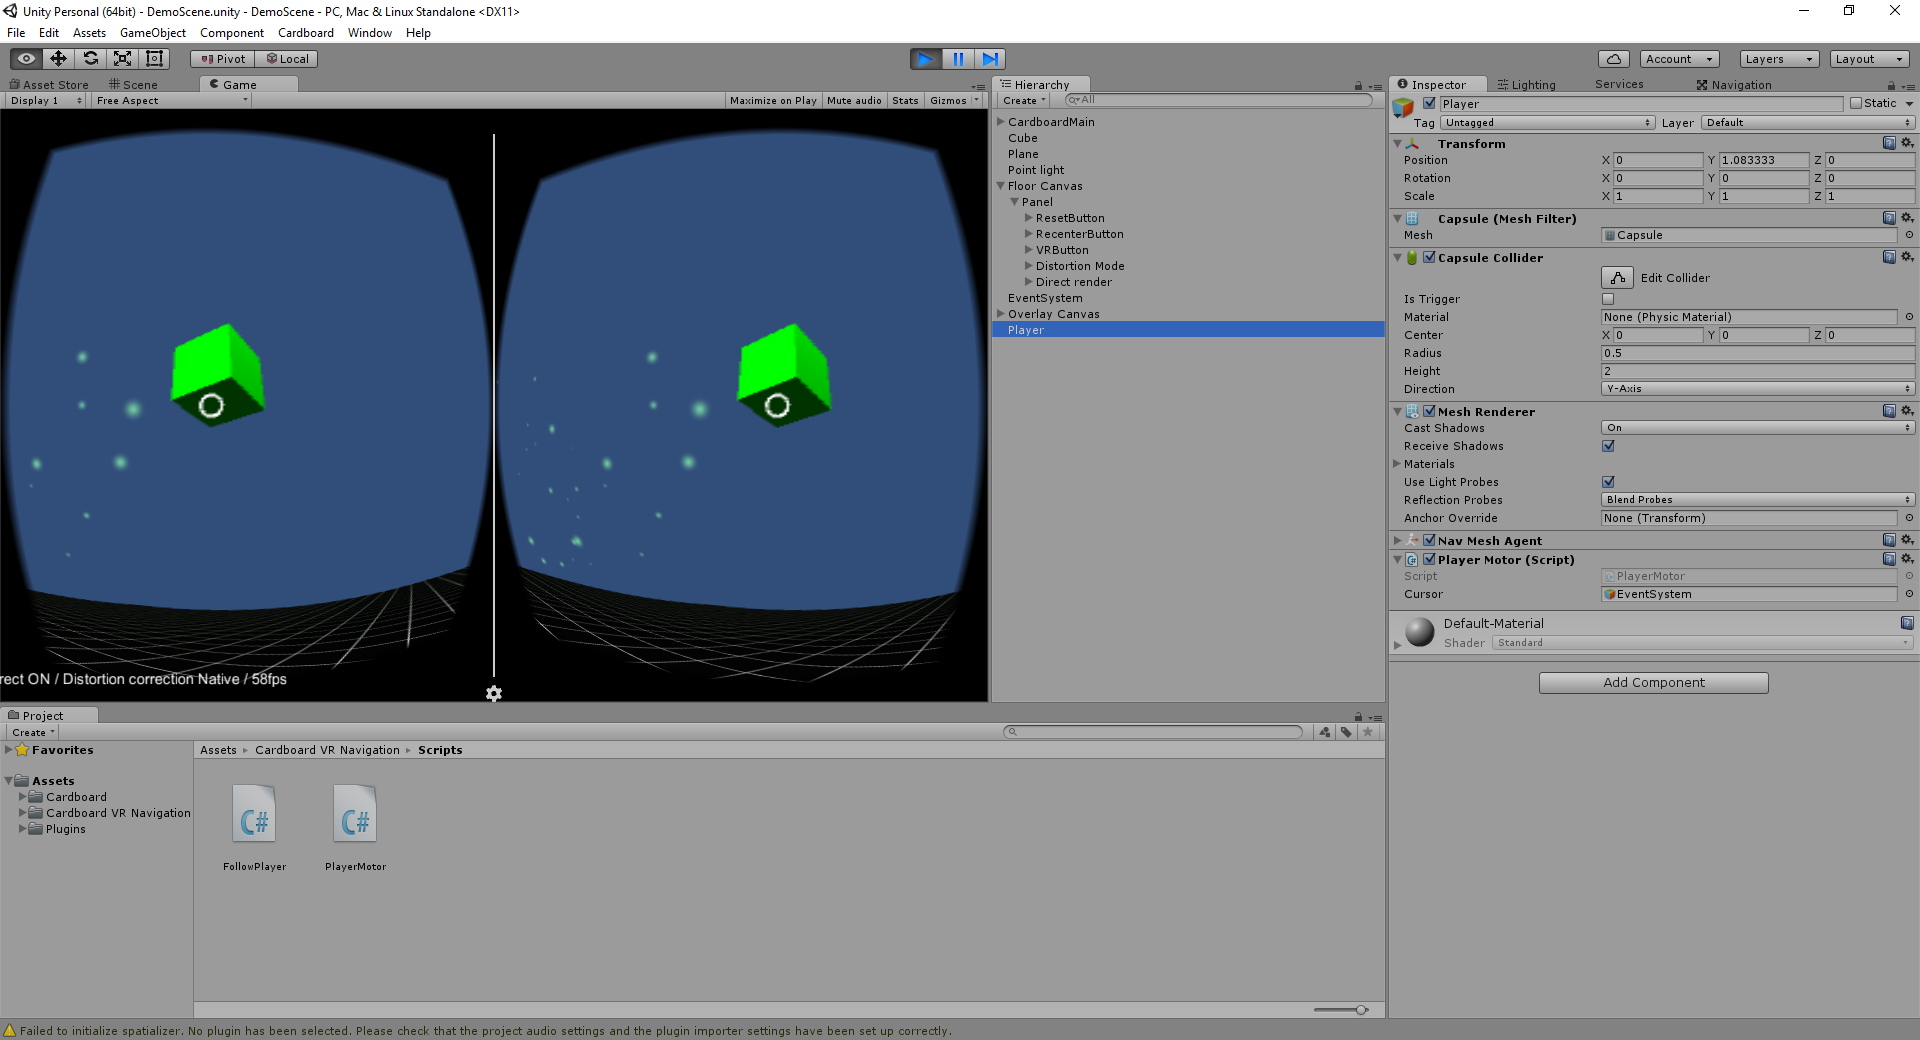
\includegraphics[width=.7\textwidth]{DemoSoftware2}
  \caption{Unity User Interface}
  \label{fig:UnityUI}
 \end{figure}

\subsubsection{Scripting}

\par Writing code in Unity is what controls the objects in the visual editor and makes the game interactive. Game objects in Unity are built as a collection of components. This collection of components often include scripts, which refer to code files. Another nice aspect of Unity is code is not compiled and run as a separate executable, but instead executed within the Unity engine itself. Being able to test your game in a separate window without the inconvenience of having to create builds is very substantial. Unity supports both Javascript and C-sharp programming languages, although C-sharp is often preferred because it is strongly typed. When it comes time for writing scripts, picking an ideal IDE or text editor is important. Unity comes bundled with MonoDevelope, which is the IDE of choice because it is open source and offers cross-platform support for C-sharp. 

\subsection{Creating VR Through Unity}

A distinct difference between VR and an average game is the fact that when immersed in a virtual environment, quality is not just how good something looks, but how good something feels. 

\subsubsection{Virtual Immersion Essentials} 

Building an environment in Unity is one thing, but turning it into virtual reality involves a few extra steps. With a VR application, different hardware is required, often with different types of input. With the Google Cardboard headset, look based techniques, an effective user interface and a first person perspective must be implemented. As mentioned previously, since the Cardboard has only one input that mimics the action of tapping on the screen, a device clicker must be created to allow for simple interactions. An additional challenge is that inputs have not yet been standardized across all platforms, meaning input devices may or may not fit under Unity's Input Manager and API's \cite{linowes}. 

 \begin{figure}[h]
    \centering
 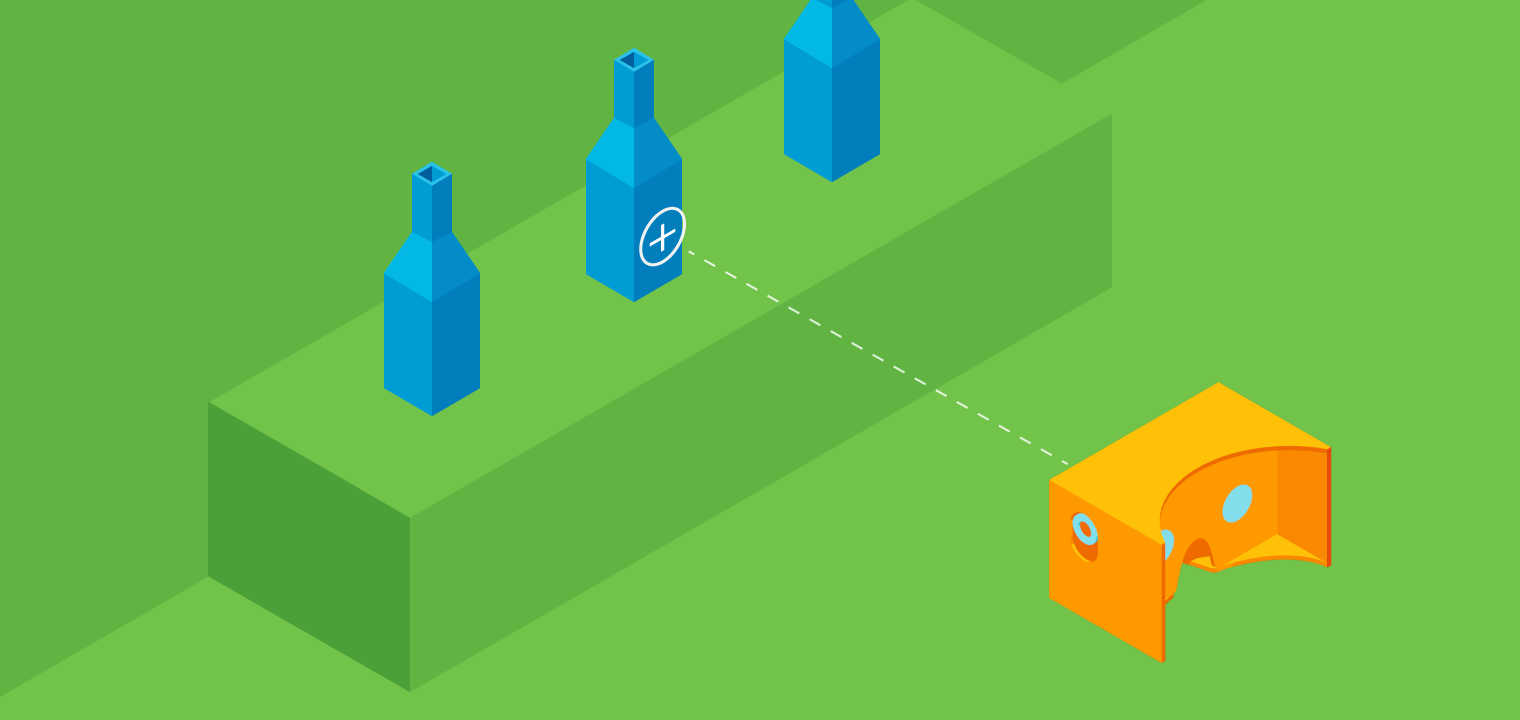
\includegraphics[width=.6\textwidth]{image13_reticle}
  \caption{Implementing A Feedback Curser \cite{reticle}}
  \label{fig:reticle}
 \end{figure}
 
\par Since many applications depend on a clicker, the position of where your gaze falls must be displayed. For this reason, a feedback cursor, or reticle, makes visible to the user where they are looking in the scene. Figure \ref{fig:reticle} illustrates how a feedback cursor is valuable for interacting with objects in a scene. Look-based techniques add dimension to a game with limited input sources, making them a must in VR development.

\par A graphical user interface (GUI) is also essential for presenting information. A GUI refers to two-dimensional on screen graphics that overlay the main gameplay and present messages, gauges, or input controls such as menus buttons or sliders \cite{linowes}. In typical non VR games, a user interface is rendered in screen space, which statically rests somewhere on the screen as an overlay, such as a screen edge. In virtual reality, there are no screen edges, and the GUI must be rendered in what is called the World Space. Some GUI's are placed at the feet of the virtual user, demonstrated in figure \ref{fig:GUI}. This style and placement for a GUI is easy to access and nonintrusive to the scene.

 \begin{figure}[h]
    \centering
 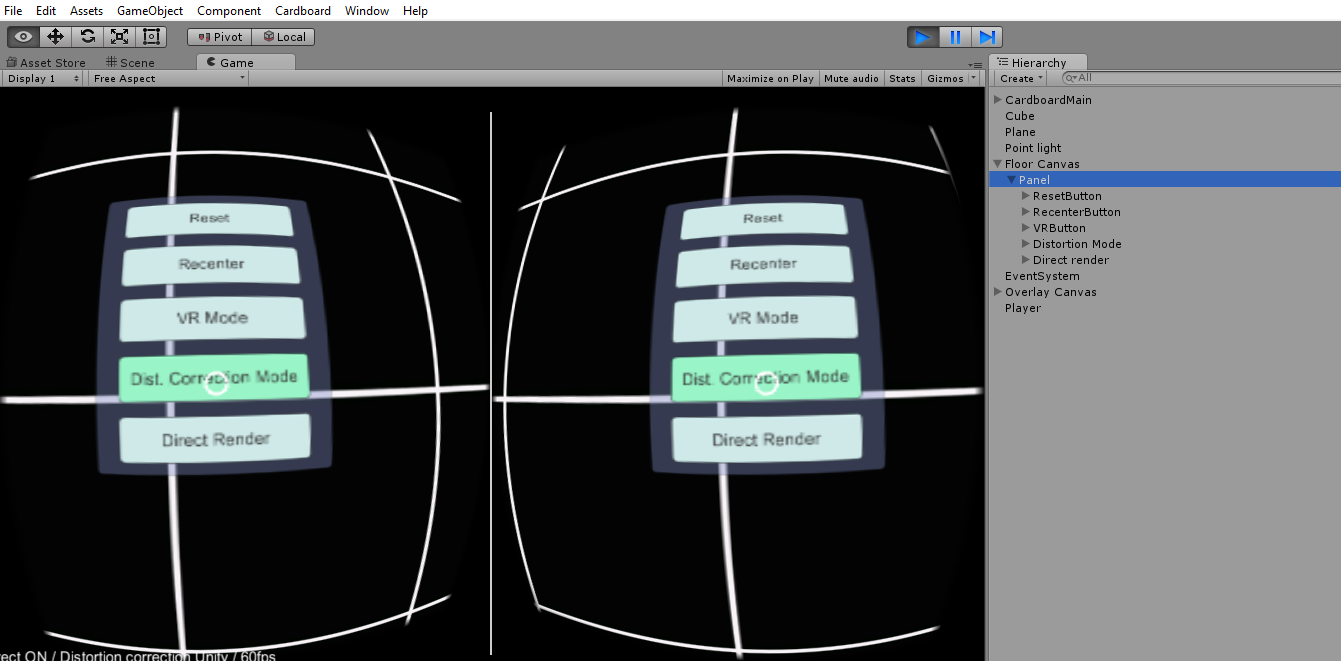
\includegraphics[width=.7\textwidth]{DemoSoftware1}
  \caption{Example of a Graphical User Interface}
  \label{fig:GUI}
 \end{figure}

%  An important aspect of virtual reality, is making the first person camera seem like it is a project of the user.


\subsubsection{VR Motion Sickness}

Despite the wonders of VR immersion, it is also known to cause feelings similar to motion sickness such as disorientation and nausea. VR motion sickness is a fairly substantial concern and is studied by many researchers, physiologists and technologists to find the underlying causes. We do know that lag caused by screen updates and synchronization problems when moving your head are a major contributing issue.
Given the potential impact rendering permanence, frames per second and latency have on a VR application, optimizing implantation and content must be at the front of any developers mind \cite{gobbetti}. 
%Spatio-temporal realism, the ability to meet synchronization, lag, and accuracy constraints within low tolerates, has therefore become a required feature for virtual reality systems . 
 Although these are the major issues corresponding to VR motion sickness, there are a few others we should consider \cite{linowes}:

\begin{enumerate}[topsep=0pt,itemsep=-1ex,partopsep=1ex,parsep=1ex]
  \item Don't move too fast.
  \item Look forwards when moving through a scene.
  \item Avoid turning head too quickly.
  \item Use a third-person camera in certain settings.
  \item Provide visual cues to keep user grounded.
  \item Provide an option to recenter the view.
  \item Cut scenes break and transitions.
  \item Optimize rendering performance wherever possible.
\end{enumerate}

 \clearpage
 


%%%%%%%%%						
%    Section 5   %
%%%%%%%%%


\section{Mobile VR Project}

\subsection{Head Mounted Display - Google Cardboard}
This project focuses on development for the Google Cardboard, a head mounted display. Other Virtual headsets such as the Oculus Rift and Gear VR are very high end, complex and pricey. These factors make owning one of these headsets unrealistic for the entry level VR enthusiast. Although these higher-end consumer products are steadily becoming more user friendly, affordable and accessible, the Google Cardboard remains the best VR option for the average consumer. Google Cardboard is a simple, low-cost VR headset for smartphones. Google released cardboard VR in 2014 with the vision that anyone with a smartphone could experience VR. The Cardboard has been very popular in the market and among developers, with hundreds of applications already available for both Android and IOS \cite{parisi}.

 \begin{figure}[h]
    \centering
 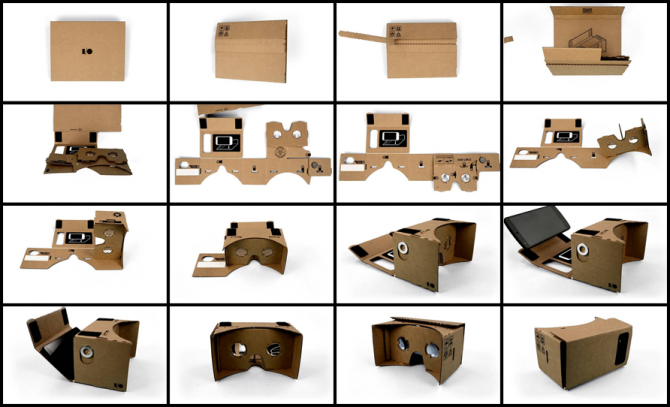
\includegraphics[width=\textwidth]{picture14_cardboard}
  \caption{Google Cardboard Setup \cite{cardboard}}
  \label{fig:cardboard}
 \end{figure}

\subsubsection{Input for the Google Cardboard}
One of Google Cardboard's biggest shortcomings is the lack of input sources. Since the smartphone is placed into the cardboard box, it is not possible to reach the screen of the phone to perform actions such as swiping or tapping. The Cardboard does, however, have a magnet mounted on the outside of the box that triggers events within an application, similar to someone tapping the screen. The only problem is the limited range of events that can be created while just having simple tapping capabilities within an app. Even though the Cardboard allows people to experience VR for a very modest price, having limited input hurts the potential for immersive experiences. To work around these limitations, manufacturers are experimenting with peripherals such as bluetooth-connected devices that would allow for simple clicking and swiping \cite{parisi}.

\subsection{Project Software}
This project used Unity to create a simple yet realistic looking scene in VR. The downloadable Cardboard SDK provides a first person camera (CardboardMain) that is implemented within the scene, shown in figure \ref{fig:maincamera}.
 \begin{figure}[h]
    \centering
 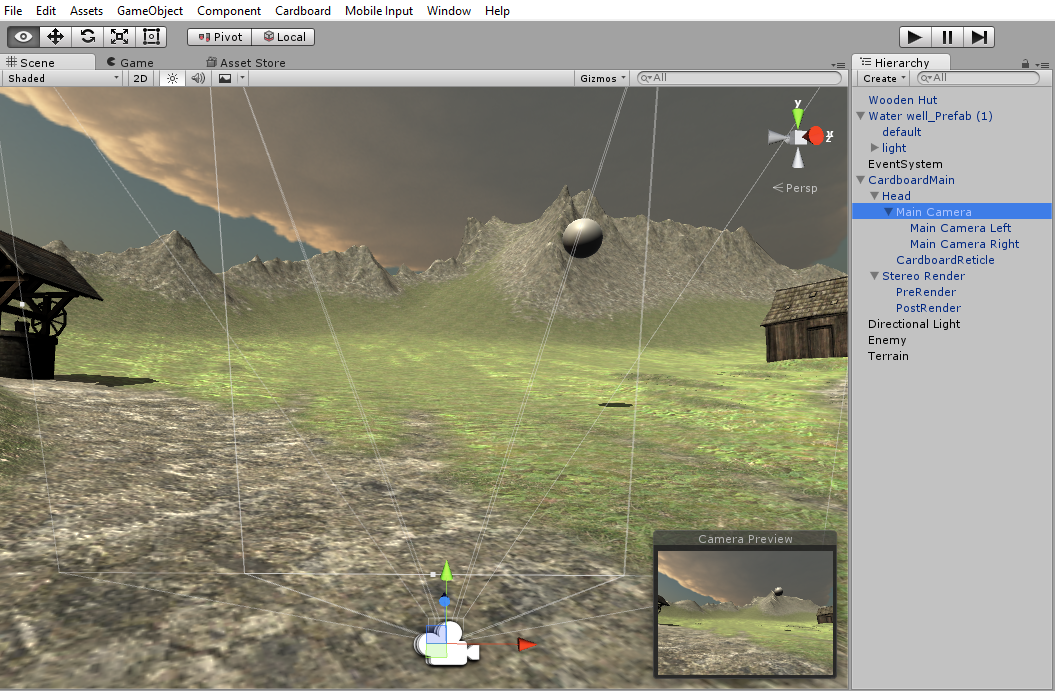
\includegraphics[width=.65\textwidth]{Software10}
  \caption{Google Cardboard Main Camera}
  \label{fig:maincamera}
 \end{figure}
The user is placed into a grassy mountain range near a small cabin and water well. The mountain terrain was imported from Unity's Asset Store. The Unity Asset Store provides developers with an array of landscape textures, terrains, skyboxes, animations, objects and characters that can be downloaded and implemented into a scene. This particular landscape is chosen % should this be was chosen??? present sounds weird here!
for it's realism and large dynamic scale, emphasized in figure \ref{fig:mountain}.  

\begin{figure}[h]
    \centering
 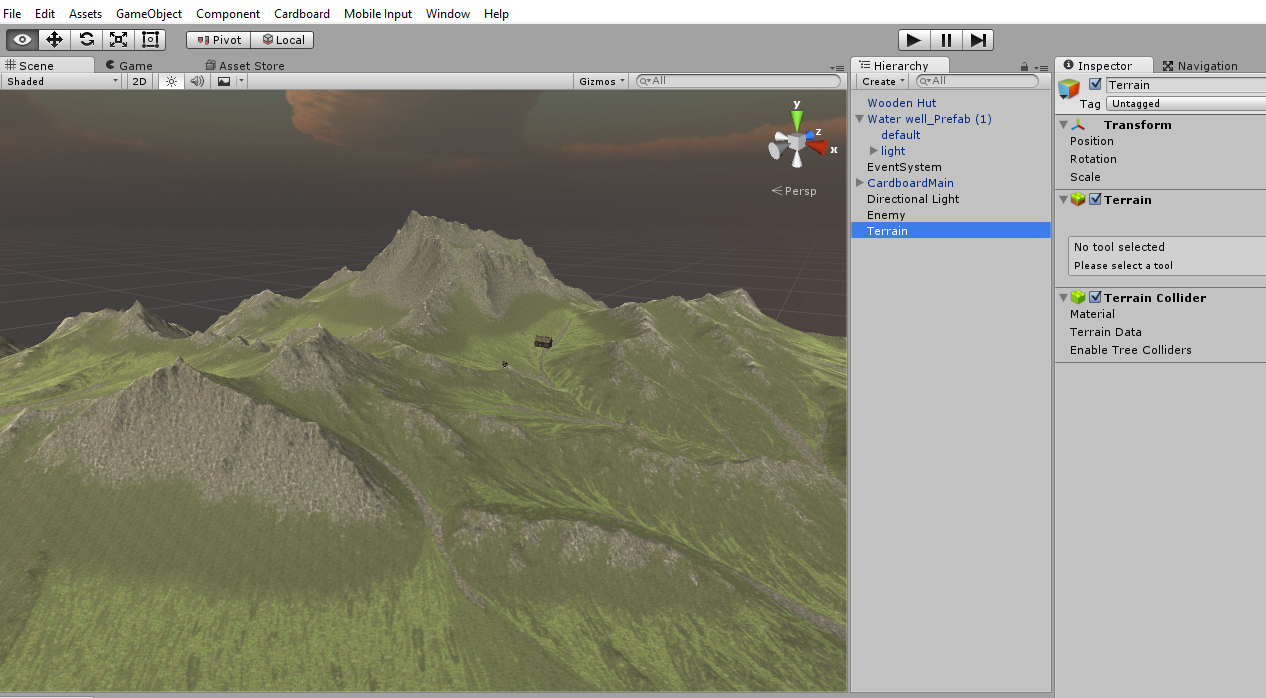
\includegraphics[width=.8\textwidth]{Software6}
  \caption{Mountain Terrain}
  \label{fig:mountain}
 \end{figure}

\par There also exists a floating ball agent that the user can direct his gaze towards and interact with using a feedback curser.
The feedback curser, or reticle, is represented on the screen as a white dot. When the reticle hovers over the ball, it widens to give the user a visual cue that the ball can be clicked. This is demonstrated in figure \ref{fig:VRreticle}. Every time the ball is clicked, it changes color and randomly moves to a new position in the scene. % talk about the diameter is moves around / more info? 
 \begin{figure}[h]
    \centering
 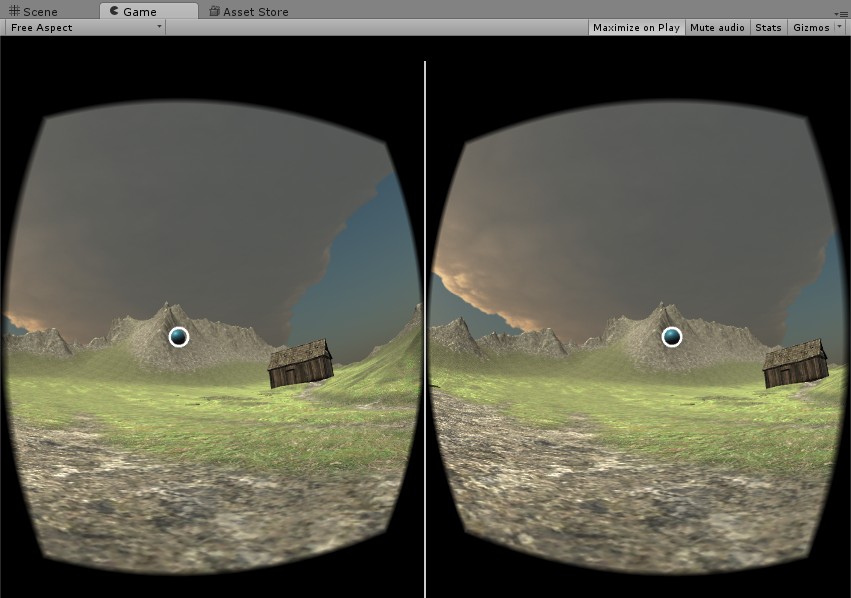
\includegraphics[width=.6\textwidth]{Software4}
  \caption{Illustration of the Google Cardboard Reticle}
  \label{fig:VRreticle}
 \end{figure}
Several components including scripts, event triggers, and a navigation mesh were implemented onto the terrain and ball to allow this movement around the scene. A RandomClick script is written and attached to the ball agent, providing the logic for it's random movement and color changes. An event trigger is implemented that calls the RandomClick script anytime the ball is clicked by the user. Finally, a navigation mesh is applied to the terrain in order for the ball to understand what areas of the terrain are acceptable for movement. In other words, a navigation mesh is a data structure that aids agents, such as the ball, in pathfinding through a complex terrain such as the mountain landscape. For example, if there exists an incline in the terrain too steep, the ball is told it can no longer continue to advance upwards. The nav mesh can be seen visually in figure \ref{fig:navMesh}

 \begin{figure}[h]
    \centering
 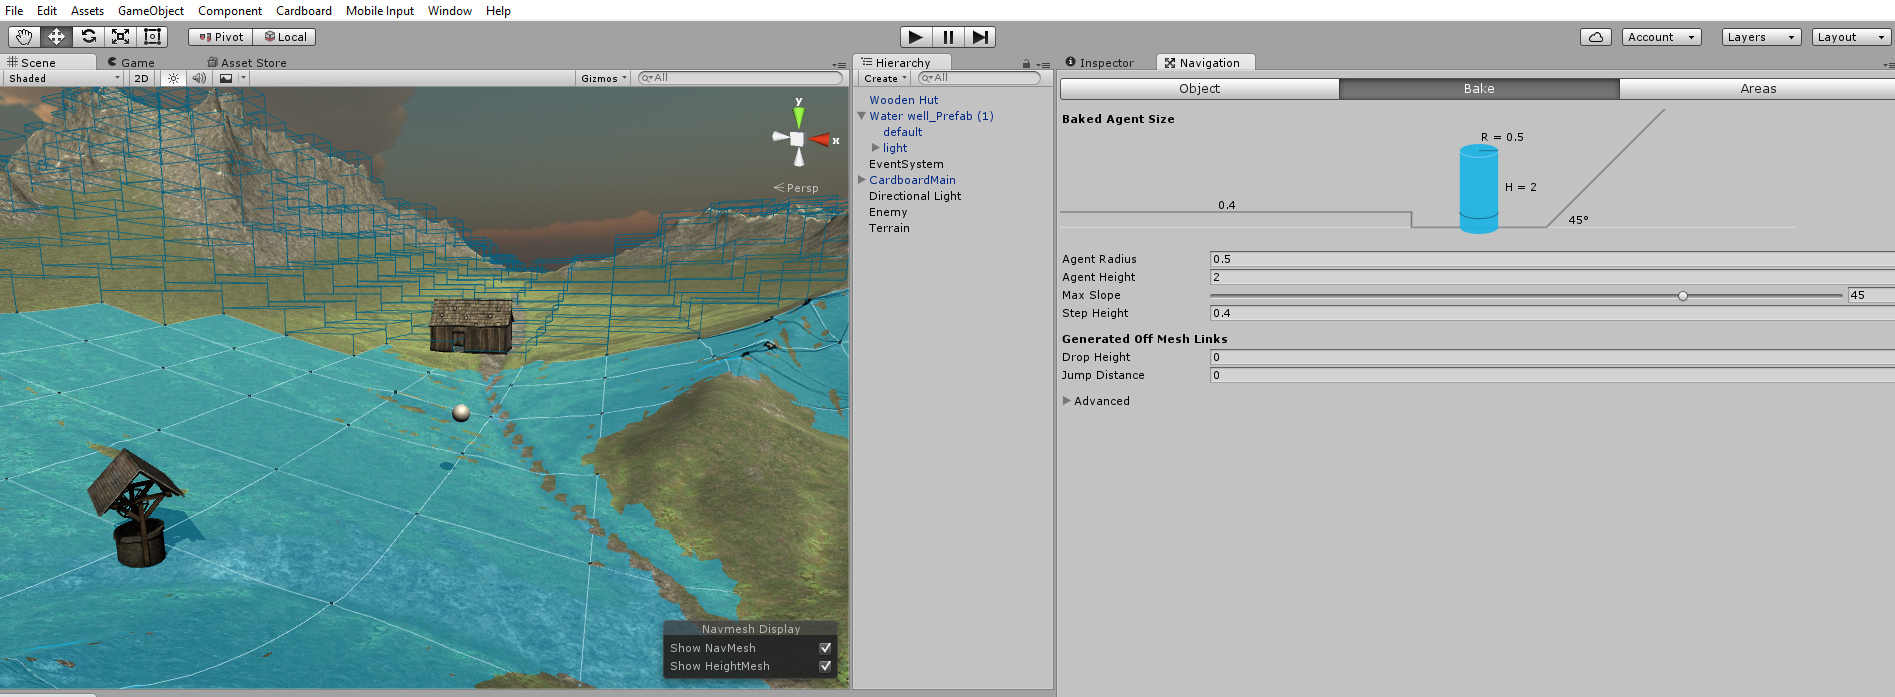
\includegraphics[width=.9\textwidth]{Software9}
  \caption{Navigation Mesh}
  \label{fig:navMesh}
 \end{figure}

% In order for this to work, a nav mesh agent componant was also added to the ball that communicated with the nav mesh the parameters of collision 

The biggest challenges were creating a terrain, placing VR camera, and implementing the components and behavior of the floating ball. However, A large and equally difficult part of this project was learning Unity and learning how to successfully export a VR application onto an external mobile device.


%%%%%%%%%						
%    Section 6   %
%%%%%%%%%

 \clearpage
 
 
\section{Conclusion}

VR is a new and expanding field. There are many areas that have come a long way, but are still less than ideal. Immersion within a VR system is one of these areas. In order to understand immersion, one must understand how the illusion of VR is created. The more senses that are stimulated and engaged, the better the immersive experience in a virtual environment. It is the virtual systems that are ultimately responsible for completing an immersive experience. There are many variables to work with to maximize virtual presence and immersion, and beginning to understand them better is the first step to creating better systems. VR may be improved in the future by creating more advanced, non-intrusive and accessible hardware. The expansion of hardware systems would allow VR to expand and be implemented in many different fields. 

\par The goal of this project was to use the theory on what makes successful immersive VR experiences and transfer that into a simple mobile VR application. The resulting project application allows a user to visually explore a fantastic mountain range right during a sunset while interacting with a colorful ball that floats around the scene. Future work would include a deeper understanding of Unity and implementing more of the theory discussed in this paper into the application.

 \begin{figure}[h]
    \centering
 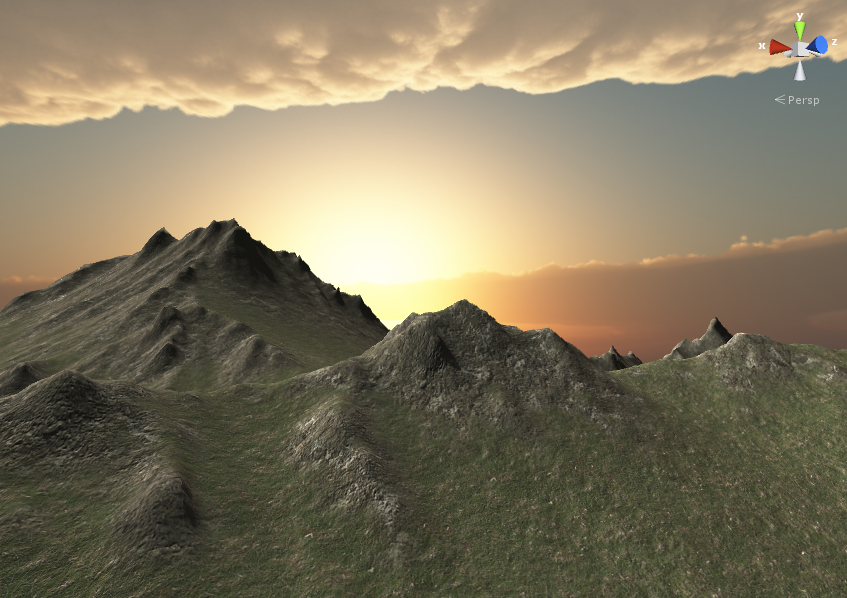
\includegraphics[width=.7\textwidth]{Software11}
  \caption{Sunset View within Application}
  \label{fig:sunset}
 \end{figure}




%Creating the illusion of virtual reality

%How the senses contribute to that illusion

%How these senses are implemented through enabling hardware. 

% virtual systems that implement human senses into the simulation

%how to display bib without citing:



\nocite{mihelj}
\nocite{okita}
\nocite{craig}
\nocite{lavieri}
\nocite{parisi}
\nocite{parisi}
\nocite{benton}
\nocite{jackson}
\nocite{blackman}
\nocite{hocking}
\nocite{linowes}
\nocite{fuchs1}
\nocite{gobbetti}

% PHOTOS

\nocite{photo1_sutehrland}
\nocite{applications}
\nocite{cardboard}
\nocite{CAVE}
\nocite{haptics}
\nocite{oculus}
\nocite{pov}
\nocite{reticle}
\nocite{sound}




\bibliographystyle{plain-annote}
\bibliography{references}

\end{document}                          % This command indicates the end of the file.
